\chapter{Conception}
This chapter presents the conceptual design of the proposed job‑matching system, which addresses the limitations identified in the previous chapters. Building on the research gap outlined in \autoref{sota:research_gap}, the goal of the conception is to translate the methodological requirements into a coherent system architecture that enables reliable requirements extraction and semantically informed similarity search. The system operates as a processing layer on top of the YourJobFinder platform, which serves as the data acquisition component by aggregating raw, unstructured job descriptions based on a user’s initial query.

\autoref{fig:yourjobfinder_architecture} illustrates the overall workflow. The YourJobFinder crawler provides raw HTML content, after which the job matching system developed in this thesis is applied. This system consists of two central components:

\begin{itemize}
    \item a requirements extraction module based on open‑source LLMs,
and
    \item an embedding‑driven similarity search module that identifies semantically relevant job postings.
\end{itemize}

(TODO: repeats the research gap promises, remove and replace by explaining what comes next) Together, these components form a lightweight, fully open‑source alternative to more resource‑intensive industrial systems, while still enabling meaningful semantic matching.

\begin{figure}[h!]
    \centering
    \includegraphics[width=1\textwidth]{images/DDD-Miro-7-11-bold}
    \caption{System architecture integrating YourJobFinder with the proposed job‑matching system.}
    \label{fig:yourjobfinder_architecture}
\end{figure}

\section{Data Structure for Job Matching}
\label{sec:data_structure}

The core of the proposed system relies on a structured comparison between job requirements and user profiles. \autoref{fig:data_structure} illustrates the fundamental data model that enables semantic matching. Both job postings and user profiles are decomposed into three key dimensions:

\begin{itemize}
    \item \textbf{Skills} — technical and professional competencies
    \item \textbf{Experience} — work history and domain expertise
    \item \textbf{Education and Certificates} — formal qualifications and certifications
\end{itemize}

These structured representations are encoded in a common Pydantic Object \cite{pydantic_validation_2025} for both job descriptions and user profiles. The requirements extraction module converts unstructured job descriptions into this schema so that they share the same structure as user profiles. With this common schema, the system can compare skills, experience, and education in a consistent way, forming the basis for the LLM extraction step and the subsequent embedding-based similarity search.

\begin{figure}[h!]
    \centering
    \includegraphics[width=0.9\textwidth]{images/requirement-user-profile-schema}
    \caption{Data structure mapping between job requirements and user profile for semantic matching.}
    \label{fig:data_structure}
\end{figure}

\section{Handling raw data}
The pipeline begins with raw HTML job postings retrieved by the YourJobFinder crawler. In their original form, these documents often contain large amounts of non‑informative content, such as JavaScript, CSS, advertisements, and unrelated boilerplate text. To create a structured and semantically meaningful input for the LLM, the HTML is converted into Markdown using the \textit{markdownify} library \cite{python-markdownify}. This preprocessing step ensures that only the textual content relevant to the job description is retained, thereby reducing noise and improving extraction quality.


\section{Schema-Guided LLM Output}
\label{sec:schema-guided}

The requirements extraction module must produce output that conforms to the predefined Pydantic schema described in \autoref{sec:data_structure}. However, LLMs may produce syntactically malformed JSON, ignore required fields, or include extraneous content that violates the schema \cite{llm-not-good-json}. To address this challenge, the system employs guided generation, a technique that constrains the LLM's output at inference time to ensure conformance with a formal specification.

The theoretical foundation for this approach is provided by Willard and Louf \cite{willard2023outlines}, who reformulate the problem of constrained text generation in terms of finite-state machines (FSMs). Their insight is that regular expressions and context-free grammars (CFGs) can be used to construct an index over the language model's vocabulary, enabling efficient determination of valid next tokens at each generation step.

\subsection{Finite-State Machine Formulation}
The approach relies on fundamental concepts from automata theory. A finite automaton (FA) is formally defined as a 5-tuple $(Q, \Sigma, \delta, q_0, F)$, where $Q$ is a finite set of states, $\Sigma$ is a finite alphabet, $\delta: Q \times \Sigma \to Q$ is the transition function, $q_0 \in Q$ is the start state, and $F \subseteq Q$ is the set of accept states \cite{sipser}. Regular expressions, which describe patterns such as digit sequences or identifiers, can be converted into equivalent finite automata that recognize exactly the strings matching the pattern \cite{willard2023outlines}.

In standard LLM inference, the model produces a probability distribution over the entire vocabulary for each token position. Guided generation modifies this process by applying a boolean mask $m$ that restricts the support of the distribution to only those tokens that are valid according to the constraints:

\begin{align*}
  \boldsymbol{\alpha} &= \operatorname{LLM}(S_t, \boldsymbol{\theta})\\
  \tilde{\boldsymbol{\alpha}} &= m(S_t) \odot \boldsymbol{\alpha}\\
  \tilde{s}_{t+1} &\sim \operatorname{Categorical}(\tilde{\boldsymbol{\alpha}})
\end{align*}

where $\boldsymbol{\alpha}$ represents the logits produced by the LLM, $m$ is the mask function, and $\odot$ denotes element-wise multiplication. The resulting masked distribution $\tilde{\boldsymbol{\alpha}}$ assigns zero probability to invalid tokens while preserving the relative probabilities of valid continuations \cite{willard2023outlines}.

The efficiency of this approach stems from pre-computing an index $\sigma: Q \to \mathcal{P}(\mathcal{V})$ that maps each FSM state $q \in Q$ to the subset of vocabulary tokens that would be accepted in that state. This index is constructed once per schema and reused across all generation calls, reducing the per-token computational cost from $\mathcal{O}(N)$ to $\mathcal{O}(1)$ on average, where $N$ is the vocabulary size \cite{willard2023outlines}.

\autoref{fig:fsm_masking} illustrates this process of sampling tokens for the regular expression \texttt{[0-9]:[0-9]}, which could represent, for example, a match score. Assume the vocabulary $\mathcal{V}$ contains only the set of strings $\{\text{"2"}, \text{"14"}\,\text{"7"}\,\text{"T"}\,\text{"\textbackslash"},\text{":"}\,\text{"="}\,\text{"i"}\}$. In the beginning, the FSM is in state $q_0$ and only tokens representing a one-digit number are valid; therefore, ``14'' and ``T'' are masked and their logits are set to zero. After sampling a valid digit, the FSM transitions to state $q_1$, where only the colon token is valid. Finally, after sampling the colon, the FSM reaches state $q_2$, where again only digit tokens are valid. At each generation step, the current FSM state determines which vocabulary tokens are valid continuations. Invalid tokens receive a mask value of zero, effectively removing them from consideration during sampling.

\begin{figure}[h!]
    \centering
    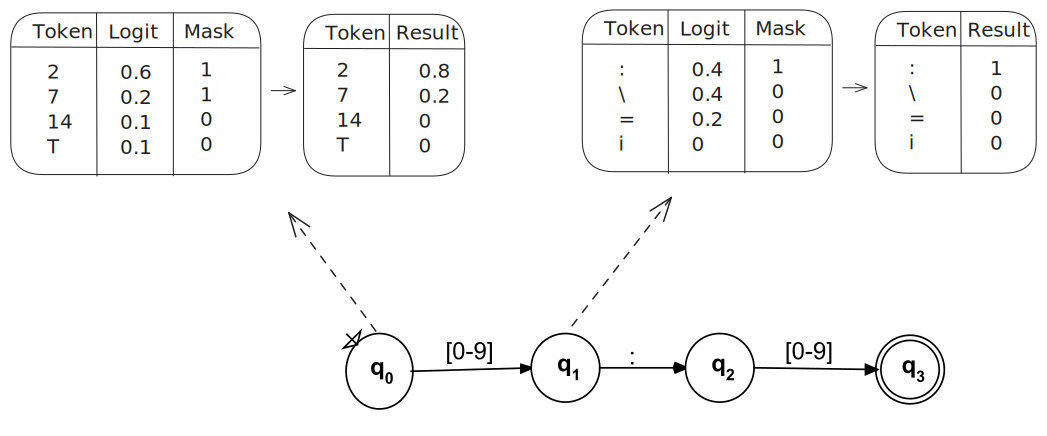
\includegraphics[width=1\textwidth]{images/outline-logits}
    \caption{FSM-guided token generation for the regular expression \texttt{[0-9]:[0-9]}. }
    \label{fig:fsm_masking}
\end{figure}


\subsection{Extension to Context-Free Grammars}
While finite automata suffice for regular languages, structured data formats such as JSON require the expressive power of context-free grammars (CFGs). CFGs can describe nested structures with arbitrary depth, such as arrays containing objects that themselves contain arrays. To recognize such languages, Willard and Louf extend their approach using pushdown automata (PDAs).

A pushdown automaton extends a finite automaton with a stack, enabling it to recognize context-free languages. Formally, a PDA is defined as a 6-tuple $(Q, \Sigma, \Gamma, \delta, q_0, F)$, where $\Gamma$ is the stack alphabet and the transition function $\delta: Q \times \Sigma_\epsilon \times \Gamma_\epsilon \to \mathcal{P}(Q \times \Gamma_\epsilon)$ additionally reads from and writes to the stack \cite{sipser}. The stack allows the automaton to remember an unbounded amount of information, which is essential for matching nested brackets and enforcing hierarchical structure. \\

In the context of this thesis, this mechanism guarantees that the extracted job requirements strictly adhere to the schema defined in \autoref{lst:requirements_schema}. By maintaining the stack configuration of the PDA, the system ensures that keys (e.g., ``experience'') are followed by valid values (e.g., arrays or strings) and that all braces and quotes are correctly closed. This eliminates the need for error-correction logic and ensures the extracted data is immediately machine-readable.

\section{LLM Models}
TODO: change this thesis  to (explain why multiple models are selected and they will be evaluated)
The thesis evaluates several state‑of‑the‑art open‑source LLMs available as of October 2025. These models were selected based on their parameter size, availability, and suitability for constrained inference environments:
\begin{table}[h]
	\caption{Model Parameter Sizes}
	\label{tab:model_params}
	\centering
	\begin{tabular}{|l|c|}
		\hline
		\textbf{Model Name} & \textbf{Parameter Size} \\
		\hline
		\hline
		Qwen3 \cite{qwen3} & 8B  \\
		\hline
		GLM-4-0414 \cite{glm2024chatglm} & 9B \\
		\hline
		mistral-7B-instruct \cite{mistral-7b} & 7B  \\
		\hline
		Llama-3.1-8B-Instruct \cite{llama-3} & 8B  \\
		\hline
	\end{tabular}
\end{table}

\section{Managing Input Data}
A limitation of Transformer-based language models is their restricted context size \cite{handson-llms-2024}, therefore to be able to process job descriptions independently of their length, the input text should be split into smaller chunks.
\subsection{Chunking Strategies}
There are different methods of chunking text data for LLM processing. It can be grouped into different categories. Following explains categories, that this work uses:
\begin{itemize}
    \item \textbf{Fixed-size chunking} It involves splitting text into chunks based on a predetermined number of tokens, with the option to include overlapping sections to preserve semantic context \cite{tamingllms}. It is widely used because it is simple, computationally inexpensive, and does not require specialized tools \cite{tamingllms}.
    \item \textbf{Structure-based chunking}: This method splits the text based on its structure and hierarchy \cite{pinecone}, In this newlines, paragraphs, or Markdown headers. This method also aims to preserve the semantic integrity of the content \cite{pinecone}.
\end{itemize}

This work uses a hybrid approach that combines the semantic preservation of structure-based chunking with the operational safety of fixed-size chunking. The primary strategy involves splitting the job descriptions by Markdown headers to maintain the coherence of logical sections. To address the limitation of variable chunk sizes, a fixed-size slicing mechanism is employed as a fallback constraint, ensuring that no single chunk exceeds the context window regardless of its structural length.

\section{LLM Output Evaluation}
Evaluating the correctness of extracted requirements poses a unique methodological challenge, as semantically equivalent requirements may be expressed in lexically diverse forms. For example, `Proven ability to manage projects simultaneously' could be correctly summarized as `Project management' . Even though the wording differs significantly.
Relying on exact string matching would thus penalize valid extractions.

To address this, the system employs an automated evaluation strategy based on the 'LLM-as-a-judge' paradigm \cite{llm-as-a-judge}. This approach uses an independent, more capable LLM to assess the faithfulness of extracted JSON fields relative to the original job
description. As Huyen mentions, ``AI judges are fast, easy to use, and relatively cheap compared to human evaluators. They can also work without reference data'' \cite{ai-engineering-book}. The evaluation framework used in this thesis is implemented with DeepEval \cite{deepeval}.

\subsection{LLM-as-a-Judge}
``The approach of using AI to evaluate AI is called AI as a judge or LLM as a judge'' \cite{ai-engineering-book}.
Evaluations may produce numeric scores or qualitative assessments \cite{blackbox-llmasjudge}. Using LLM-as-a-Judge is not just cost-effective, `` Studies have shown that certain AI judges are strongly correlated to human evaluators.'' \cite{ai-engineering-book}. Zheng et al. found in their work that LLM judges and humans can achieve 85\% agreement, while the agreement among human evaluators was 81\% \cite{llm-as-a-judge}.


\subsection{G-Eval} \label{conception:g-eval}
The evaluation relies on the G‑Eval metric, a prompt‑based scoring method with three components: (1) task definition and criteria, (2) a chain‑of‑thought reasoning process used internally by the judge model, and (3) a probabilistic scoring function \cite{G-eval}. This mechanism enables controlled and interpretable evaluation of structured JSON outputs.

\subsection{Metrics} \label{metrics}
Four criteria adapted from Yuan et al. \cite{evaluation-mertric} guide the evaluation:

\begin{itemize}
    \item \textbf{Correctness} — assesses whether extracted requirements are accurate and present in the input text.
    \item \textbf{Completeness} — evaluates whether all mandatory requirements have been captured.
    \item \textbf{Alignment} — measures whether the model avoids including `preferred', `bonus', or non‑mandatory requirements.
    \item \textbf{Readability} — examines whether the output adheres to the defined schema and is syntactically valid.
\end{itemize}
These metrics collectively ensure that extraction quality is judged not only by semantic fidelity but also by structural reliability.

\section{Embedding and Similarity Search}
Once the job requirements have been extracted and validated, the second component of the system performs semantic similarity matching. Both the structured job postings and the user query are encoded as vector
representations using the \textit{all‑MiniLM‑L6‑v2} sentence transformer model. As discussed in \autoref{introduction:similaritysearch}, this model offers strong zero‑shot performance for retrieval‑based tasks in job matching.\\
The skills fields are weighted more because as studies show skills are more important in job application, for example a study by Bone et al. , that analysed online job postings from 2018 to 2024, points out ``We show that individual skills, rather than formal education requirements, have become increasingly important features of job advertisements for AI roles.'' \cite{skills-or-degree}.

Task of similarity search is to give a similarity score by embedding the extracted requirements and user profile, which have the same structure and comparing them using maxsim approach.

\subsection{Vector Embedding}
An embedding effectively maps discrete objects, like words or documents, to points in a continuous vector space \cite{llm-from-scratch}. \autoref{fig:embeddings-process} illustrates this transformation from raw input to a vector representation, which serves as a good way to translate human language into computer language. \cite{handson-llms-2024}

\begin{figure}[h!]
    \centering
    \includegraphics[width=0.8\textwidth]{images/embeddings-process}
    \caption{the process of converting raw data into a three-dimensional numerical vector (Source: \cite{llm-from-scratch}).}
    \label{fig:embeddings-process}
\end{figure}

Embeddings are fixed in size, with their values representing various properties that collectively capture the meaning of a word in a way that is interpretable by a computer \cite{handson-llms-2024}. A key advantage of using embeddings is the ability to measure semantic similarity. By calculating distance metrics in the vector space, it is possible to determine how closely related two words are; words sharing similar meanings tend to be clustered closer together \cite{handson-llms-2024}, \autoref{fig:embeddings-distances} illustrates how words with similar meaning tend to be closer to each other, if it was possible to compress the embeddings into a two-dimensional representation \cite{handson-llms-2024}.

\begin{figure}[h!]
    \centering
    \includegraphics[width=0.8\textwidth]{images/embeddings-distances}
    \caption{Embeddings of words that are similar will be close to each other in dimensional space (Source: \cite{handson-llms-2024}).}
    \label{fig:embeddings-distances}
\end{figure}

\subsection{MaxSim} \label{subsec:maxsim}

Computing a meaningful similarity score between extracted job requirements and a user profile is non-trivial. A naive pairwise comparison fails because lists often differ in length and items may appear in different orders. To address this, this thesis adopts a matching strategy inspired by the MaxSim framework originally introduced by Chan and Ng \cite{maxsim} for machine translation evaluation.

In the original MaxSim paper, the authors utilize the Kuhn-Munkres algorithm to find a maximum weight matching in a bipartite graph, ensuring a strict 1-to-1 alignment between items. In contrast, this thesis employs a row-wise maximum aggregation over the similarity matrix. This modification is a deliberate design choice: in job matching, the number of requirements often exceeds the number of profile items, and a single broad competency in a user profile may semantically satisfy multiple specific job requirements.

The algorithm proceeds in the following steps:
\begin{enumerate}
    \item \textbf{Embedding:} Both the job requirements $J = \{j_1, \dots, j_n\}$ and user attributes $U = \{u_1, \dots, u_m\}$ are mapped to a high-dimensional vector space.
    \item \textbf{Similarity Matrix:} A similarity matrix $C$ is computed, where each entry $C_{ik}$ represents the cosine similarity between the $i$-th job requirement and the $k$-th user profile item.
    \item \textbf{Max-Over-Rows Aggregation:} For every specific job requirement $j_i$, the system identifies the maximum similarity score found across all user items $U$:
\end{enumerate}

The similarity score for a specific data field (e.g., Skills) is defined as the mean of these maximum satisfaction scores:

\begin{equation} \label{eq:maxsim_coverage}
    Score_{field} = \frac{1}{|J|} \sum_{i=1}^{|J|} \max_{k} (C_{ik})
\end{equation}

\begin{figure}[h!]
    \centering
    \includegraphics[width=0.8\textwidth]{images/maxsim-matrix}
    \caption{Visualization of the similarity matrix. The system identifies strong semantic alignment (green cells) between user skills and job requirements, even when exact wording differs.}
    \label{fig:maxsim_matrix}
\end{figure}

In the context of \autoref{fig:maxsim_matrix}, the calculation would proceed as follows:
\begin{itemize}
    \item Requirement \textit{Python}: Max match is 1.0 (from User: Python).
    \item Requirement \textit{Java}: Max match is 0.4 (from User: Python).
    \item Requirement \textit{Teamwork}: Max match is 0.8 (from User: Team player).
\end{itemize}
The final score for this section would be the average of these maximums: $(1.0 + 0.4 + 0.8) / 3 \approx 0.73$.


This approach ensures that every job requirement is evaluated against the user's best matching attribute, effectively measuring how much of the job description is ``covered'' by the user's profile.

\subsection{Weighted Field Aggregation}
Recognizing that not all data categories hold equal value in recruitment, the system segments the comparison into three dimensions: \textit{Skills}, \textit{Experiences}, and \textit{Qualifications}. The final semantic match score is a weighted linear combination of these field scores:

\begin{equation}
    Score_{total} = w_{skills} \cdot Score_{skills} + w_{exp} \cdot Score_{exp} + w_{qual} \cdot Score_{qual}
\end{equation}

By assigning higher weights to skills, the model aligns with recent findings on the increasing importance of skills-based hiring as explained above.
